\let\negmedspace\undefined
\let\negthickspace\undefined
\documentclass[journal]{IEEEtran}
\usepackage[a5paper, margin=10mm, onecolumn]{geometry}
%
\setlength{\headheight}{1cm} % Set the height of the header box
\setlength{\headsep}{0mm}     % Set the distance between the header box and the top of the text

\usepackage{gvv-book}
\usepackage{gvv}
\usepackage{cite}
\usepackage{amsmath,amssymb,amsfonts,amsthm}
\usepackage{algorithmic}
\usepackage{graphicx}
\usepackage{textcomp}
\usepackage{xcolor}
\usepackage{txfonts}
\usepackage{listings}
\usepackage{enumitem}
\usepackage{mathtools}
\usepackage{gensymb}
\usepackage{comment}
\usepackage[breaklinks=true]{hyperref}
\usepackage{tkz-euclide} 
\usepackage{listings}
% \usepackage{gvv}                                        
\def\inputGnumericTable{}                                 
\usepackage[latin1]{inputenc}                                
\usepackage{color}                                            
\usepackage{array}                                            
\usepackage{longtable}                                       
\usepackage{calc}                                             
\usepackage{multirow}                                          
\usepackage{hhline}                                           
\usepackage{ifthen}                                           
\usepackage{lscape}

\begin{document}
	
	\bibliographystyle{IEEEtran}
	\vspace{3cm}
	\title{10.3.4.2.4}
	\author{EE24BTECH11022 - ESHAN SHARMA}
	% \maketitle
	% \newpage
	{\let\newpage\relax\maketitle}
	
	\renewcommand{\thefigure}{\theenumi}
	\renewcommand{\thetable}{\theenumi}
	\setlength{\intextsep}{10pt} % Space between text and floats
	
	
	\numberwithin{equation}{enumi}
	\numberwithin{figure}{enumi}
	\renewcommand{\thetable}{\theenumi}
	
	\textbf{Question:}
	Meena went to a bank to withdraw 2000. She asked the cashier to give her 50 and 100 notes only. Meena got 25 notes in all. Find how many notes of 50 and 100 she received.\\
	
	\textbf{Solution:}
	
	\textbf{Step 1: Form the system of linear equations}\\
	Let the number of 50 notes be \(x\) and the number of 100 notes be \(y\). From the problem, we form the following equations:
	\begin{align}
		x + y &= 25 \quad \text{(1)} \\
		50x + 100y &= 2000 \quad \text{(2)}
	\end{align}
	
	\textbf{Step 2: Represent the system in matrix form}\\
	The system of equations can be written as:
	\[
	A \mathbf{x} = \mathbf{b}
	\]
	where
	\[
	A = \begin{pmatrix} 1 & 1 \\ 50 & 100 \end{pmatrix}, \quad \mathbf{x} = \begin{pmatrix} x \\ y \end{pmatrix}, \quad \mathbf{b} = \begin{pmatrix} 25 \\ 2000 \end{pmatrix}.
	\]
	
	\textbf{Step 3: Perform LU decomposition using Doolittle's algorithm}\\
	The LU decomposition splits \(A\) into a lower triangular matrix \(L\) and an upper triangular matrix \(U\) such that:
	\[
	A = LU
	\]
	where:
	\[
	L = \begin{pmatrix} 1 & 0 & 0 & \cdots & 0 \\ l_{21} & 1 & 0 & \cdots & 0 \\ l_{31} & l_{32} & 1 & \cdots & 0 \\ \vdots & \vdots & \vdots & \ddots & 0 \\ l_{n1} & l_{n2} & l_{n3} & \cdots & 1 \end{pmatrix}, \quad
	U = \begin{pmatrix} u_{11} & u_{12} & u_{13} & \cdots & u_{1n} \\ 0 & u_{22} & u_{23} & \cdots & u_{2n} \\ 0 & 0 & u_{33} & \cdots & u_{3n} \\ \vdots & \vdots & \vdots & \ddots & u_{n-1,n} \\ 0 & 0 & 0 & \cdots & u_{nn} \end{pmatrix}.
	\]
	
	The Doolittle algorithm is computed as follows:
	
	1. For \(U\):
	\[
	u_{ij} = a_{ij} - \sum_{k=1}^{i-1} l_{ik} u_{kj}, \quad \text{for } i \leq j.
	\]
	
	2. For \(L\):
	\[
	l_{ij} = \frac{1}{u_{ii}} \left(a_{ij} - \sum_{k=1}^{i-1} l_{ik} u_{kj} \right), \quad \text{for } i > j.
	\]
	
	3. Diagonal entries of \(L\) are set to 1:
	\[
	l_{ii} = 1, \quad \text{for all } i.
	\]
	
	Using these general formulas, we compute \(L\) and \(U\) for our specific problem:
	\[
	A = \begin{pmatrix} 1 & 1 \\ 50 & 100 \end{pmatrix}.
	\]
	\textbf{Step 3.1: Compute the elements of \(L\) and \(U\)}\\
	\begin{align}
		u_{11} &= a_{11} = 1, \quad u_{12} = a_{12} = 1 \\
		l_{21} &= \frac{a_{21}}{u_{11}} = \frac{50}{1} = 50 \\
		u_{22} &= a_{22} - l_{21}u_{12} = 100 - 50 \cdot 1 = 50
	\end{align}
	
	Thus, the matrices \(L\) and \(U\) are:
	\[
	L = \begin{pmatrix} 1 & 0 \\ 50 & 1 \end{pmatrix}, \quad U = \begin{pmatrix} 1 & 1 \\ 0 & 50 \end{pmatrix}.
	\]
	
	\textbf{Step 4: Solve the system using forward and backward substitution}\\
	First, solve \(L \mathbf{y} = \mathbf{b}\) for \(\mathbf{y}\):
	\[
	\begin{pmatrix} 1 & 0 \\ 50 & 1 \end{pmatrix} \begin{pmatrix} y_1 \\ y_2 \end{pmatrix} = \begin{pmatrix} 25 \\ 2000 \end{pmatrix}.
	\]
	This gives:
	\begin{align}
		y_1 &= 25, \\
		50y_1 + y_2 &= 2000 \quad \Rightarrow \quad 50(25) + y_2 = 2000 \quad \Rightarrow \quad y_2 = 750.
	\end{align}
	Thus, \(\mathbf{y} = \begin{pmatrix} 25 \\ 750 \end{pmatrix}\).
	
	Next, solve \(U \mathbf{x} = \mathbf{y}\) for \(\mathbf{x}\):
	\[
	\begin{pmatrix} 1 & 1 \\ 0 & 50 \end{pmatrix} \begin{pmatrix} x \\ y \end{pmatrix} = \begin{pmatrix} 25 \\ 750 \end{pmatrix}.
	\]
	This gives:
	\begin{align}
		50y &= 750 \quad \Rightarrow \quad y = 15, \\
		x + y &= 25 \quad \Rightarrow \quad x + 15 = 25 \quad \Rightarrow \quad x = 10.
	\end{align}
	
	\textbf{Solution:}\\
	The number of 50 notes is \(x = 10\), and the number of 100 notes is \(y = 15\).
	
	\textbf{Step 5: Plot the lines and show the intersection point}\\
	The lines representing the equations are:
	\begin{align}
		x + y &= 25, \\
		50x + 100y &= 2000.
	\end{align}
	
	The intersection point of these lines is \((10, 15)\).
	
	\begin{figure}[h]
		\centering
		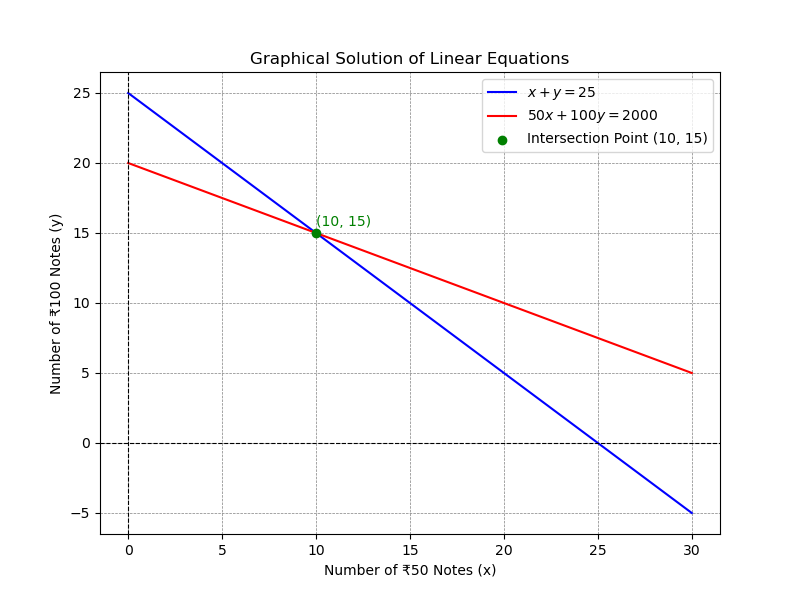
\includegraphics[width=\textwidth]{figs/fig.png}
	\end{figure}
	
	\textbf{Conclusion:}\\
	Meena received 10 notes of 50 and 15 notes of 100. This satisfies both the total number of notes (25) and the total amount withdrawn (2000).
	
	
\end{document}
